\chapter{单细胞生物的多样性}\label{ch:b2:unicellular-diversity}

显微镜下的一滴池塘水中，有一个绿色细胞借两根鞭毛
划动，一个拖鞋形的纤毛虫把细菌扫进自己的胞口，
一个透明的硅藻沿载玻片滑动，还有一千个
细菌，太小而难以看清。每个都是一个细胞，也都是一个完整的
生物体：它以单个细胞的形式摄食、运动、感知、生长、繁殖和死亡。
生物世界的大部分始终如此。本章把\omterm{def:b2:unicellular-diversity:unicellular}{单细胞生物}
视为一个设计问题——即一个细胞能做什么、
不能做什么——并考察\omterm{def:b2:unicellular-diversity:prokaryote}{原核生物}与真核生物所找到的各种答案，
直到细胞开始聚在一起
为止。

\section{一个细胞，全部功能}

\begin{definition}[单细胞、群体与多细胞]\label{def:b2:unicellular-diversity:unicellular}
生物体称为\emph{单细胞生物}\index{单细胞生物}，当其单个细胞
承担生命的全部功能——营养、交换、运动、繁殖，
并能独立生活。生物体称为
\emph{群体生物}\index{群体生物}，当同一种类的细胞分裂后仍相连，
但每个细胞若被分开，都仍能独立生存。生物体称为
\emph{多细胞生物}\index{多细胞生物}，当其细胞属于若干类型、彼此依赖，
且只有其中少数细胞（生殖细胞系）留下后代。
单细胞生物包括全部古菌、几乎全部细菌，
以及大多数真核生物谱系；非正式名称\emph{\omterm{def:b2:unicellular-diversity:protist}{原生生物}}
泛指单细胞真核生物，它们并非单一类群，
而是许多类群。
\end{definition}

\begin{example}[一滴水中的六种居民]\label{ex:b2:unicellular-diversity:drop}
\emph{Escherichia coli}，一种长 \qty{2}{\micro m} 的杆菌，借一簇鞭毛
游动，营养充足时每二十分钟分裂一次。
\emph{Chlamydomonas}，一种直径 \qty{10}{\micro m} 的绿藻，借两根鞭毛
划动，朝着其眼点所感知的光游动。
\emph{Paramecium}，一种大小为 \qty{200}{\micro m} 的纤毛虫，体表覆盖
数千根纤毛，借胞口摄食，并用两个\omterm{prop:b2:unicellular-diversity:osmoregulation}{伸缩泡}向外排水。
一种硅藻生活在由二氧化硅构成的两片式壳中，壳上带孔纹。
\emph{Amoeba} 借伸出伪足而流动，
并吞噬所遇到的一切。一个酵母细胞\omterm{def:b2:unicellular-diversity:division}{出芽}，
从一侧生出子细胞。六种答案，大小与结构差异悬殊，
都是对同一问题的回答。
\end{example}

\begin{omfigure}
\begin{tikzpicture}[x=1.9cm]
  % log scale from 0.1 um to 100 mm : position = log10(size in um) + 1
  \draw[thick] (0,0) -- (6,0);
  \foreach \p/\l in {0/{\qty{0.1}{\micro m}},1/{\qty{1}{\micro m}},2/{\qty{10}{\micro m}},3/{\qty{100}{\micro m}},4/{\qty{1}{mm}},5/{\qty{10}{mm}},6/{\qty{100}{mm}}}
    \draw (\p,0.12) -- (\p,-0.12) node[below, font=\scriptsize] {\l};
  \foreach \p/\c/\l in {0.5/omDef/支原体, 1.3/omDef/{\emph{E.~coli}}, 1.7/omDef/酵母, 2.0/omProp/{\emph{Chlamydomonas}}, 2.7/omProp/硅藻, 3.3/omProp/{\emph{Paramecium}}, 3.65/omProp/{\emph{Amoeba proteus}}, 3.9/omThm/{\emph{Thiomargarita}（一种细菌）}, 5.7/omProp/{\emph{Acetabularia}}}
    { \fill[\c] (\p,0) circle (0.05); \node[rotate=60, anchor=west, font=\scriptsize, \c, inner sep=1pt] at (\p,0.12) {\l}; }
  \node[font=\scriptsize, anchor=north] at (3,-0.55) {细胞大小（对数刻度）};
\end{tikzpicture}

{\small \omterm{def:b2:unicellular-diversity:unicellular}{单细胞生物}的大小跨越五个数量级。\omterm{def:b2:unicellular-diversity:prokaryote}{原核生物}（蓝色）
集中在一微米左右；真核细胞（橙色）
大十到一百倍。体积最大的单个细胞——巨型硫细菌
与藻类 \emph{Acetabularia}——
均为正文将加以说明的例外。}
\end{omfigure}

\begin{proposition}[表面积、体积与大小的限制]\label{prop:b2:unicellular-diversity:surface}
\index{表面积与体积之比}
细胞通过其表面与外界交换物质，
消耗量与其体积成正比。对于半径为 $r$ 的球体，
其\emph{\omterm{prop:b2:unicellular-diversity:surface}{表面积与体积之比}}为
\[
\frac{S}{V} = \frac{4\pi r^2}{\tfrac{4}{3}\pi r^3} = \frac{3}{r},
\]
因此半径加倍时，每单位细胞质可利用的表面积
减半。依靠细胞膜扩散向内部供给营养的细胞，
因而不能无限生长：达到某一半径后，经表面的供应
便不再满足体积的需求。同一规律也解释了为何小细胞
单位质量的代谢最活跃，
以及大细胞为何呈扁平、伸长之状，
或带有液泡，或充满内膜。
\end{proposition}

\begin{theorem}[扩散一段距离所需的时间]\label{thm:b2:unicellular-diversity:diffusion}
\index{扩散时间}
扩散系数为 $D$ 的分子做随机步运动；
经过时间 $t$ 后，其沿某一轴的均方位移为
$\langle x^2\rangle = 2Dt$。仅靠扩散覆盖距离 $x$
所需的时间因此为
\[
t \approx \frac{x^2}{2D},
\]
该时间随距离的\emph{平方}增长。取
水中小分子的扩散系数 $D \approx \qty{1e-9}{m^2/s}$，穿越
一个细菌（\qty{1}{\micro m}）需半毫秒；穿越一个
\qty{1}{mm} 的细胞需八分钟，而穿越一米则需十六
年。
\end{theorem}
\begin{proof}
设分子每步长为 $\ell$，随机地向左或向右迈步，
每 $\tau$ 秒迈一步。经过 $n$ 步后，其位移为
$x = \sum_i \varepsilon_i \ell$，其中 $\varepsilon_i = \pm 1$
相互独立，因此 $\langle x\rangle = 0$，且 $\langle x^2\rangle =
\sum_i \langle\varepsilon_i^2\rangle \ell^2 = n\ell^2$（交叉
项的平均为零）。代入 $n = t/\tau$ 得 $\langle x^2\rangle
= (\ell^2/\tau)\,t$，记 $D = \ell^2/2\tau$，则
$\langle x^2\rangle = 2Dt$。令 $\langle x^2\rangle = x^2$，即得
所需时间。
\end{proof}

\begin{theorem}[球形细胞的扩散供应]\label{thm:b2:unicellular-diversity:supply}
\index{扩散受限的摄取}
半径为 $r_0$ 的球形细胞，吸收每一个
抵达其表面的溶质分子，置于远处浓度为
$c_\infty$ 的介质中，稳态时接收的
通量（每秒分子数）为
\[
J = 4\pi D r_0\, c_\infty .
\]
供应仅随 $r_0$ 增长，而需求随
$r_0^3$ 增长：超过某一半径后，依靠扩散获取营养的细胞将会饥饿。
\end{theorem}
\begin{proof}
稳态时，穿过每个
半径为 $r > r_0$ 的球面的每秒分子数相同，即 $J = 4\pi r^2 D\,
(\mathrm{d}c/\mathrm{d}r)$（由菲克定律，通量指向内侧）。
因此 $r^2\,\mathrm{d}c/\mathrm{d}r = J/4\pi D$ 为常数；积分
自 $r_0$（此处 $c = 0$）积分至无穷远（此处 $c = c_\infty$）：
$c_\infty = (J/4\pi D)\int_{r_0}^{\infty} r^{-2}\,\mathrm{d}r =
J/(4\pi D r_0)$，于是 $J = 4\pi D r_0 c_\infty$。
\end{proof}

\begin{example}[依靠扩散供养的细胞能有多大？]\label{ex:b2:unicellular-diversity:howbig}
一个需氧细胞消耗氧气的速率约为 $q = \qty{0.02}{mol/m^3/s}$
（以每单位细胞质体积计，这是较快的速率）。其需求为 $q \cdot \tfrac{4}{3}\pi
r_0^3$；空气饱和水提供的供应（$c_\infty =
\qty{0.25}{mol/m^3}$，$D = \qty{2e-9}{m^2/s}$）为 $4\pi D r_0
c_\infty$。令二者相等，$r_0^2 = 3Dc_\infty/q = 3\times 2\times 10^{-9}
\times 0.25/0.02 = \qty{7.5e-8}{m^2}$，故 $r_0 \approx
\qty{270}{\micro m}$。实际活跃的细胞远小于此值，因为
氧气还必须扩散到细胞\emph{内部}；\qty{750}{\micro m}
的硫细菌\emph{Thiomargarita}通过使自身几乎全部为液泡而绕过限制，
其细胞质形成一层薄壳，
厚仅几微米。
\end{example}

\begin{omfigure}
\begin{tikzpicture}
\begin{axis}[
  width=0.8\linewidth, height=6.2cm,
  axis x line=bottom, axis y line=left,
  xmode=log, ymode=log,
  xmin=0.3, xmax=1000, ymin=1e-6, ymax=1e4,
  xlabel={细胞半径 (\unit{\micro m})}, ylabel={每秒分子数（相对值）},
  xlabel style={font=\small, at={(axis description cs:0.5,-0.1)}, anchor=north},
  ylabel style={font=\small},
  tick label style={font=\small},
  legend style={font=\small, at={(0.03,0.97)}, anchor=north west, draw=none},
  clip=false,
]
\addplot[very thick, omDef, domain=0.3:1000, samples=40] {x/10};
\addlegendentry{扩散供应，$\propto r$}
\addplot[very thick, omThm, domain=0.3:1000, samples=40] {(x/10)^3/1000*1.0};
\addlegendentry{细胞质需求，$\propto r^3$}
\draw[dashed, gray] (axis cs:270,1e-6) -- (axis cs:270,27);
\node[font=\scriptsize, anchor=west] at (axis cs:300,3e-4) {饥饿半径};
\end{axis}
\end{tikzpicture}

{\small 经表面的供应随 $r$ 增长，需求随
$r^3$ 增长（对数坐标）。两线相交处，仅靠扩散供养的细胞
已无法使其内部得到供应；
交点约在数百微米处，对活跃的需氧细胞而言，
即为这类细胞的极限尺寸。}
\end{omfigure}

\section{原核生物多样性}

\begin{definition}[原核细胞]\label{def:b2:unicellular-diversity:prokaryote}
\emph{原核生物}\index{原核生物}（细菌和古菌，两个域彼此之间的差别
与它们各自同我们之间的差别一样大）是一种
没有细胞核、也没有膜包被细胞器的细胞：具有一条单条
环状染色体位于\emph{拟核}\index{拟核}中，常常还带有
称为\emph{质粒}\index{质粒}的小型额外环状DNA，核糖体游离于
细胞质中（尺度为 \qtyrange{0.5}{2}{\micro m}），质膜
带有呼吸链或光合链，还有坚硬的
\emph{细胞壁}\index{细胞壁!细菌的}，用以抵抗
细胞质中比外界高出数个巴的膨压。形态种类不多，
且各有专名：\emph{球菌}（球形）、\emph{杆菌}（杆状），
\emph{螺菌}和\emph{螺旋体}（螺旋形）、\emph{弧菌}
（逗号形）；分裂后，细胞可能成对、成链、成四联体或成簇
存在。
\end{definition}

\begin{proposition}[双层包膜：革兰氏阳性与革兰氏阴性]\label{prop:b2:unicellular-diversity:gram}
\index{革兰氏染色}\index{肽聚糖}
细菌的\omterm{def:b2:unicellular-diversity:prokaryote}{细胞壁}由\emph{\omterm{prop:b2:unicellular-diversity:gram}{肽聚糖}}构成，即由两种交替排列的糖
经短肽交联而成的链，在细胞周围连成一个巨大的
分子。\emph{革兰氏阳性菌}具有较厚的
一层（\qtyrange{20}{80}{nm}），位于单层膜外侧，并保留
\omterm{prop:b2:unicellular-diversity:gram}{革兰氏染色}过程中的结晶紫染料；\emph{革兰氏阴性菌}
具有一层薄的（仅几纳米）\omterm{prop:b2:unicellular-diversity:gram}{肽聚糖}，夹在质膜与
\emph{外膜}之间，外膜的外小叶由
脂多糖构成，因此不保留染料。外
膜上镶嵌有孔蛋白，构成第二道屏障：它能阻挡许多
抗生素和去污剂，这正是革兰氏阴性菌感染
较难治疗的原因。古菌既无\omterm{prop:b2:unicellular-diversity:gram}{肽聚糖}，也没有
其他细胞所具有的酯键连接的脂质：其膜由
醚键连接的类异戊二烯链构成，有时贯穿整个
双层膜，形成单分子层，使其能在沸腾的酸中保持稳定。
\end{proposition}

\begin{omfigure}
\begin{tikzpicture}[scale=0.9, every node/.style={font=\scriptsize}]
  % Gram-positive
  \begin{scope}
    \fill[omDef!15] (0,0) rectangle (4,1.6);
    \node at (2,0.4) {细胞质};
    \fill[omDef!60] (0,1.6) rectangle (4,1.85);
    \node[right] at (4.05,1.72) {质膜};
    \fill[omProp!50] (0,1.85) rectangle (4,3.0);
    \foreach \y in {2.0,2.25,...,2.85} \draw[omProp!90!black] (0.1,\y) -- (3.9,\y);
    \node[right, align=left] at (4.05,2.45) {厚肽聚糖层 \\(\qtyrange{20}{80}{nm})};
    \node[above, font=\small\bfseries] at (2,3.05) {革兰氏阳性};
  \end{scope}
  % Gram-negative
  \begin{scope}[xshift=7.6cm]
    \fill[omDef!15] (0,0) rectangle (4,1.6);
    \node at (2,0.4) {细胞质};
    \fill[omDef!60] (0,1.6) rectangle (4,1.85);
    \node[right] at (4.05,1.72) {质膜};
    \fill[omProp!50] (0,2.05) rectangle (4,2.25);
    \draw[omProp!90!black] (0.1,2.15) -- (3.9,2.15);
    \node[right] at (4.05,2.15) {薄肽聚糖层};
    \node at (2,1.95) {周质};
    \fill[omThm!50] (0,2.55) rectangle (4,2.85);
    \foreach \x in {0.6,2.0,3.4} \fill[white] (\x-0.12,2.55) rectangle (\x+0.12,2.85);
    \node[right] at (4.05,2.7) {带孔蛋白的外膜};
    \foreach \x in {0.2,0.5,...,3.9} \draw[omThm!80!black, thick] (\x,2.85) -- (\x,3.1);
    \node[right] at (4.05,3.15) {脂多糖};
    \node[above, font=\small\bfseries] at (2,3.3) {革兰氏阴性};
  \end{scope}
\end{tikzpicture}

{\small 两种细菌包膜的剖面示意。左：一层膜，外覆厚\omterm{prop:b2:unicellular-diversity:gram}{肽聚糖}层。
右：两层膜之间的周质中为一层薄\omterm{prop:b2:unicellular-diversity:gram}{肽聚糖}层，
外层膜上嵌有孔蛋白，
并覆有脂多糖。}
\end{omfigure}

\begin{proposition}[细菌鞭毛与趋化性]\label{prop:b2:unicellular-diversity:flagellum}
\index{鞭毛!细菌}\index{趋化性}
细菌\emph{鞭毛}是由鞭毛蛋白构成的刚性螺旋丝，
直径为 \qty{20}{nm}，长度可达数个菌体长，
由嵌在包膜中的旋转马达驱动。马达的驱动力并非来自 ATP，
而是来自质子沿跨膜电化学梯度的流动，
每转一圈约有 \num{1000} 个质子通过，
转速可达每秒 \num{300} 转。在 \emph{E.~coli} 中，多根鞭毛同时逆时针转动时束集在一起，
推动细胞沿直线前进，即\emph{游动}；
当一根或多根鞭毛反转时，鞭毛束散开，
细胞发生\emph{翻滚}，转向一个新的随机方向。\emph{\omterm{prop:b2:unicellular-diversity:flagellum}{趋化性}}是这种随机游走的偏向：细胞测定
过去一秒内引诱剂浓度是否升高，
细胞通过比较当前与最近的过去来确定方向——
即沿自身路径比较——
因为在自身 \qty{1}{\micro m} 的长度内，
测不出任何浓度梯度。
\end{proposition}
\begin{proof}[证据]
贝格与布朗（1972 年）用三维跟踪显微镜追踪了单个 \emph{E.~coli} 细胞：
游动约持续一秒，速度为 \qty{20}{\micro m/s}，
翻滚约持续十分之一秒；
在丝氨酸梯度中，朝向梯度的游动更长，
而背向梯度的游动并未缩短。将细胞通过一根鞭毛固定在玻片上，
整个菌体便会旋转，这证明马达是旋转式的；
马达与 ATP 合成脱偶联的细胞，
只要能人为建立质子梯度，仍能游动，
由此确定了能量来源。
\end{proof}

\begin{omfigure}
\begin{tikzpicture}[every node/.style={font=\scriptsize}]
  % run and tumble path without gradient
  \begin{scope}
    \draw[very thick, omDef] (0,0) -- (1.2,0.5) -- (0.7,1.4) -- (1.9,1.8) -- (2.6,0.9) -- (3.4,1.5) -- (3.0,2.5);
    \foreach \p in {(1.2,0.5),(0.7,1.4),(1.9,1.8),(2.6,0.9),(3.4,1.5)} \fill[omThm] \p circle (0.06);
    \node[align=center] at (1.8,-0.5) {无梯度：\\游动长度相等，转向随机};
  \end{scope}
  \begin{scope}[xshift=6cm]
    \shade[left color=white, right color=omExo!50] (-0.3,-0.2) rectangle (5.2,3.0);
    \draw[very thick, omDef] (0,0.3) -- (0.9,0.8) -- (0.6,1.3) -- (2.4,1.5) -- (2.2,2.2) -- (4.6,2.4);
    \foreach \p in {(0.9,0.8),(0.6,1.3),(2.4,1.5),(2.2,2.2)} \fill[omThm] \p circle (0.06);
    \node[align=center] at (2.4,-0.5) {引诱剂向右增加：\\朝向梯度的游动更长};
    \node[anchor=south east] at (5.1,2.6) {引诱剂更多};
  \end{scope}
\end{tikzpicture}

{\small 游动与翻滚。左：无梯度时，细胞进行随机游走，
每段游动（蓝色）以一次翻滚（红点）结束。右：当
沿游动方向引诱剂浓度升高时，翻滚被抑制，游动延长，
游走逐渐向梯度方向漂移。}
\end{omfigure}

\begin{example}[蓝细菌与异形胞]\label{ex:b2:unicellular-diversity:cyanobacteria}
蓝细菌是像植物一样进行光合作用的细菌，
它们在层叠的内膜上分解水并释放氧气，
（类囊体，叶绿体即由其演化而来）。许多蓝细菌
以共用一个鞘的细胞丝形式生长。在 \emph{Anabaena} 中，
当可利用的结合态氮耗尽时，约每十个细胞便有一个
转变为\emph{异形胞}：它拆除产氧的光系统，
加厚\omterm{def:b2:unicellular-diversity:prokaryote}{细胞壁}以隔绝氧气，并借助一种会被氧气破坏的酶固定大气中的氮，
同时将谷氨酰胺输送给相邻细胞，
换取糖类。\emph{Anabaena} 的一条细胞丝
是细胞间分工的初步雏形。
\end{example}

\begin{omfigure}
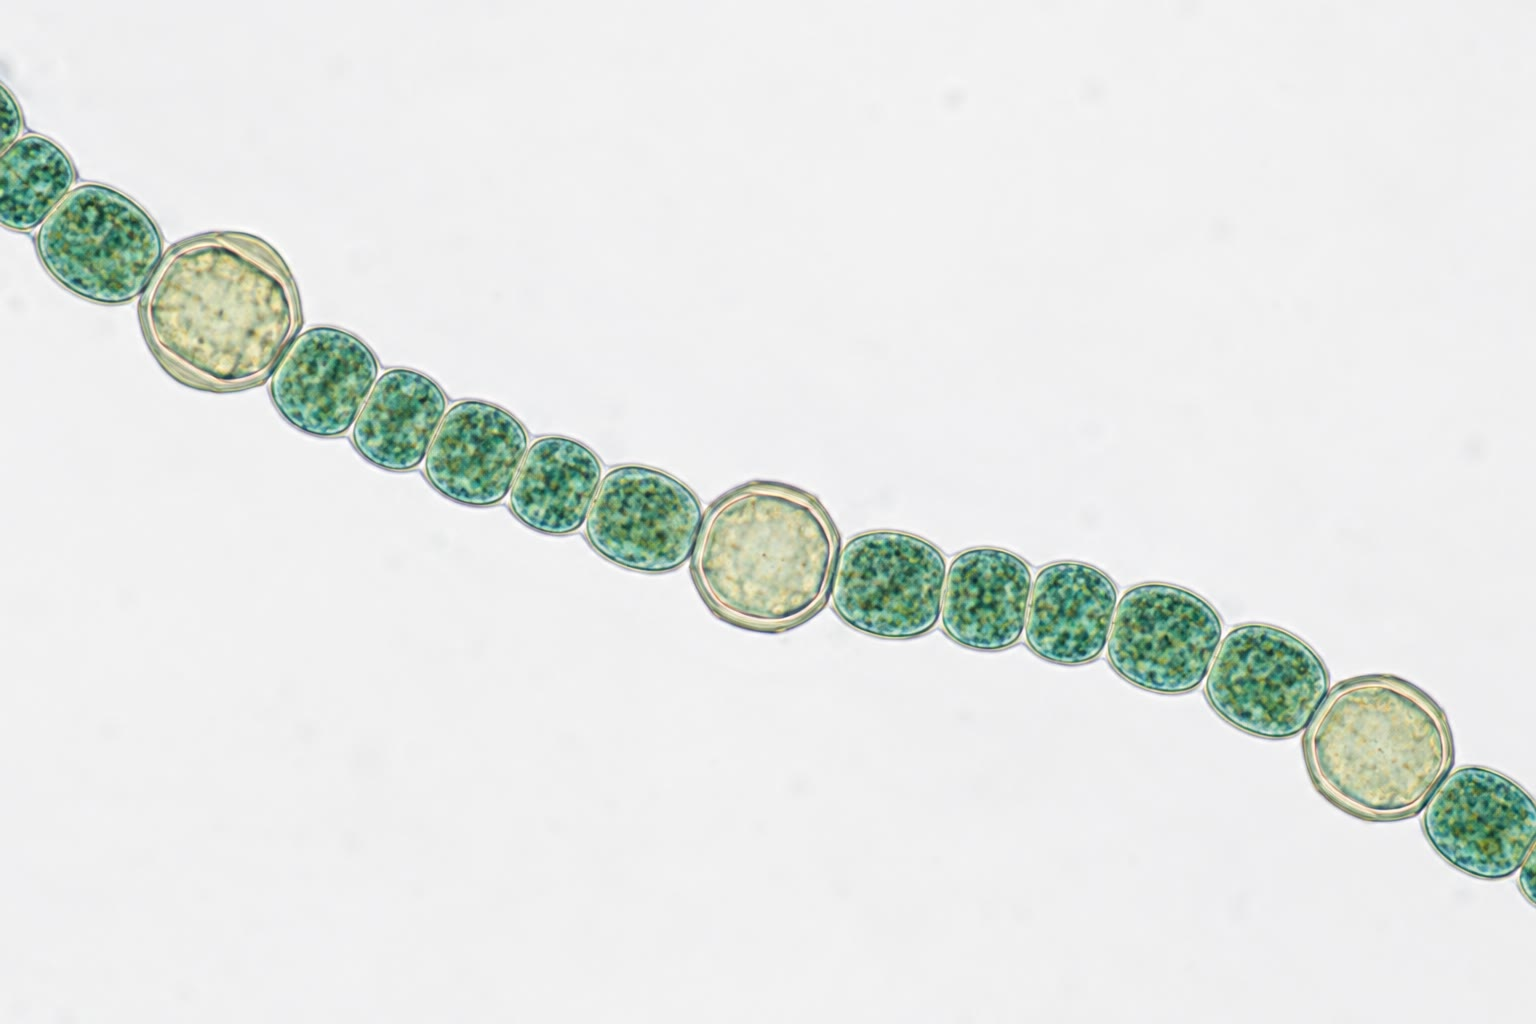
\includegraphics[width=0.62\linewidth]{images/book4/ai/b4-01-anabaena.jpg}

{\small \emph{Anabaena} 的一条细胞丝：一串绿色的光合细胞，
中间间隔着较大、颜色较浅的异形胞，
即固氮的细胞。}
\end{omfigure}

\begin{remark}[休眠]\label{rem:b2:unicellular-diversity:spores}
一些革兰氏阳性杆菌（\emph{Bacillus}、\emph{Clostridium}）在饥饿时
会形成\emph{内生孢子}：内生孢子是染色体的一个拷贝，
外包多层脱水的外壳，代谢上处于惰性状态，
能耐受煮沸、辐射以及长达数百年的干旱，
待条件恢复时萌发。许多\omterm{def:b2:unicellular-diversity:protist}{原生生物}则以\emph{孢囊}实现同样的作用。
休眠与运动并列，
是度过不利季节的另一种方式。
\end{remark}

\section{真核单细胞生物}

\begin{definition}[原生生物：一个等级，而非一个类群]\label{def:b2:unicellular-diversity:protist}
\emph{原生生物}\index{原生生物}是既非动物、也非陆生植物或真菌的真核生物——
大多为单细胞，部分为群体，少数（如海带类）为多细胞。
它们共有本科一年级分册中所述的真核细胞结构（细胞核、线粒体、内膜系统、细胞骨架、$9+2$ 型纤毛），
除此之外并无其他共同特征：
包含它们的各个谱系彼此之间的距离，
与动物和植物之间的距离相当。
绿藻与陆生植物同属一支；硅藻和褐藻各自构成一个谱系；
纤毛虫、甲藻与疟原虫构成另一谱系；
变形虫和黏菌则与动物、真菌的亲缘关系
比与上述任何一类都更近。
该词指的是一种组织层次——单独生活的真核细胞——
而不是系统树上的一个分支。
\end{definition}

\begin{example}[单独生活的真核细胞的四种方式]\label{ex:b2:unicellular-diversity:four}
\emph{Chlamydomonas}：一种卵形绿藻，\omterm{def:b2:unicellular-diversity:prokaryote}{细胞壁}为不含纤维素的糖蛋白壁，
含一个杯状叶绿体，一个橙色眼点遮蔽光感受器，
使细胞在旋转时能判断光的方向，
前端两根鞭毛以蛙泳式摆动；它是一种光能营养生物。
\emph{Paramecium}：一种纤毛虫，全身纤毛协调地呈波状摆动，
一条类似口腔的口沟将细菌扫入食物泡，有两个\omterm{prop:b2:unicellular-diversity:osmoregulation}{伸缩泡}，
并具有两种细胞核——较小的\emph{生殖小核}和
较大的\emph{营养大核}，每个基因在大核中有数百个拷贝；
它是一种\omterm{def:b2:unicellular-diversity:nutrition}{吞噬营养}生物。\emph{Amoeba}：没有\omterm{def:b2:unicellular-diversity:prokaryote}{细胞壁}，没有固定形状，
依靠肌动蛋白聚合推出的\emph{伪足}进行运动和摄食。
硅藻：一个光合细胞被两片相互重叠的硅质壳包围，
壳的形状如盒子和盒盖，
壳上布满小孔，
以至于这种壳曾被用来检验显微镜镜头；
分裂时，每个子细胞保留一片旧壳，
并在内侧合成一片新的、较小的壳。
\end{example}

\begin{omfigure}
\begin{tikzpicture}[every node/.style={font=\scriptsize}]
  % Paramecium outline (slipper)
  \draw[thick, fill=omProp!8] plot[smooth cycle, tension=0.8] coordinates {(0,0) (1.5,0.9) (3.5,1.1) (5.5,0.7) (6.4,0) (5.5,-0.8) (3.5,-1.1) (1.5,-0.9)};
  % cilia
  \foreach \t in {3,9,...,357} {
    \pgfmathsetmacro{\cx}{3.2+3.25*cos(\t)}
    \pgfmathsetmacro{\cy}{1.08*sin(\t)}
    \pgfmathsetmacro{\dx}{3.2+3.55*cos(\t)}
    \pgfmathsetmacro{\dy}{1.32*sin(\t)}
    \draw[gray] (\cx,\cy) -- (\dx,\dy);
  }
  % macronucleus and micronucleus
  \draw[thick, fill=omDef!40] (3.2,0.05) ellipse (0.9 and 0.45);
  \fill[omDef!90!black] (2.4,0.55) circle (0.13);
  % oral groove and gullet
  \draw[thick, omThm] (4.3,-0.95) .. controls (3.6,-0.5) and (3.3,-0.2) .. (3.0,-0.35);
  \fill[omThm!30] (2.9,-0.45) circle (0.16);
  % food vacuoles
  \foreach \p in {(1.4,-0.3),(1.0,0.35),(4.8,0.35)} \draw[thick, omExo!80!black, fill=omExo!30] \p circle (0.17);
  % contractile vacuoles
  \foreach \c in {(1.2,0.0),(5.2,-0.2)} {
    \draw[thick, omDef] \c circle (0.28);
    \foreach \a in {0,60,...,300} \draw[omDef] \c ++(\a:0.28) -- ++(\a:0.22);
  }
  % labels
  \draw (2.4,0.55) -- (2.7,1.6) node[above] {小核};
  \draw (3.6,0.3) -- (4.8,1.6) node[above] {大核};
  \draw (1.2,0.28) -- (0.3,1.5) node[above, align=center] {伸缩泡 \\（带放射管）};
  \draw (5.2,-0.48) -- (6.5,-1.5) node[below] {伸缩泡};
  \draw (4.3,-0.95) -- (4.7,-1.75) node[below] {口沟};
  \draw (2.9,-0.61) -- (2.7,-1.6) node[below, align=center] {胞咽与形成中 \\的食物泡};
  \draw (1.4,-0.47) -- (0.0,-1.5) node[below] {食物泡};
  \draw (6.35,0.4) -- (6.9,1.2) node[above, align=center] {纤毛};
\end{tikzpicture}

{\small \emph{Paramecium}，示意图：纤毛覆盖的皮层、
两个细胞核、通向胞咽的口沟（食物泡在此形成），
以及两个星形的\omterm{prop:b2:unicellular-diversity:osmoregulation}{伸缩泡}，用于排出
渗透作用带入的水分。}
\end{omfigure}

\begin{omfigure}
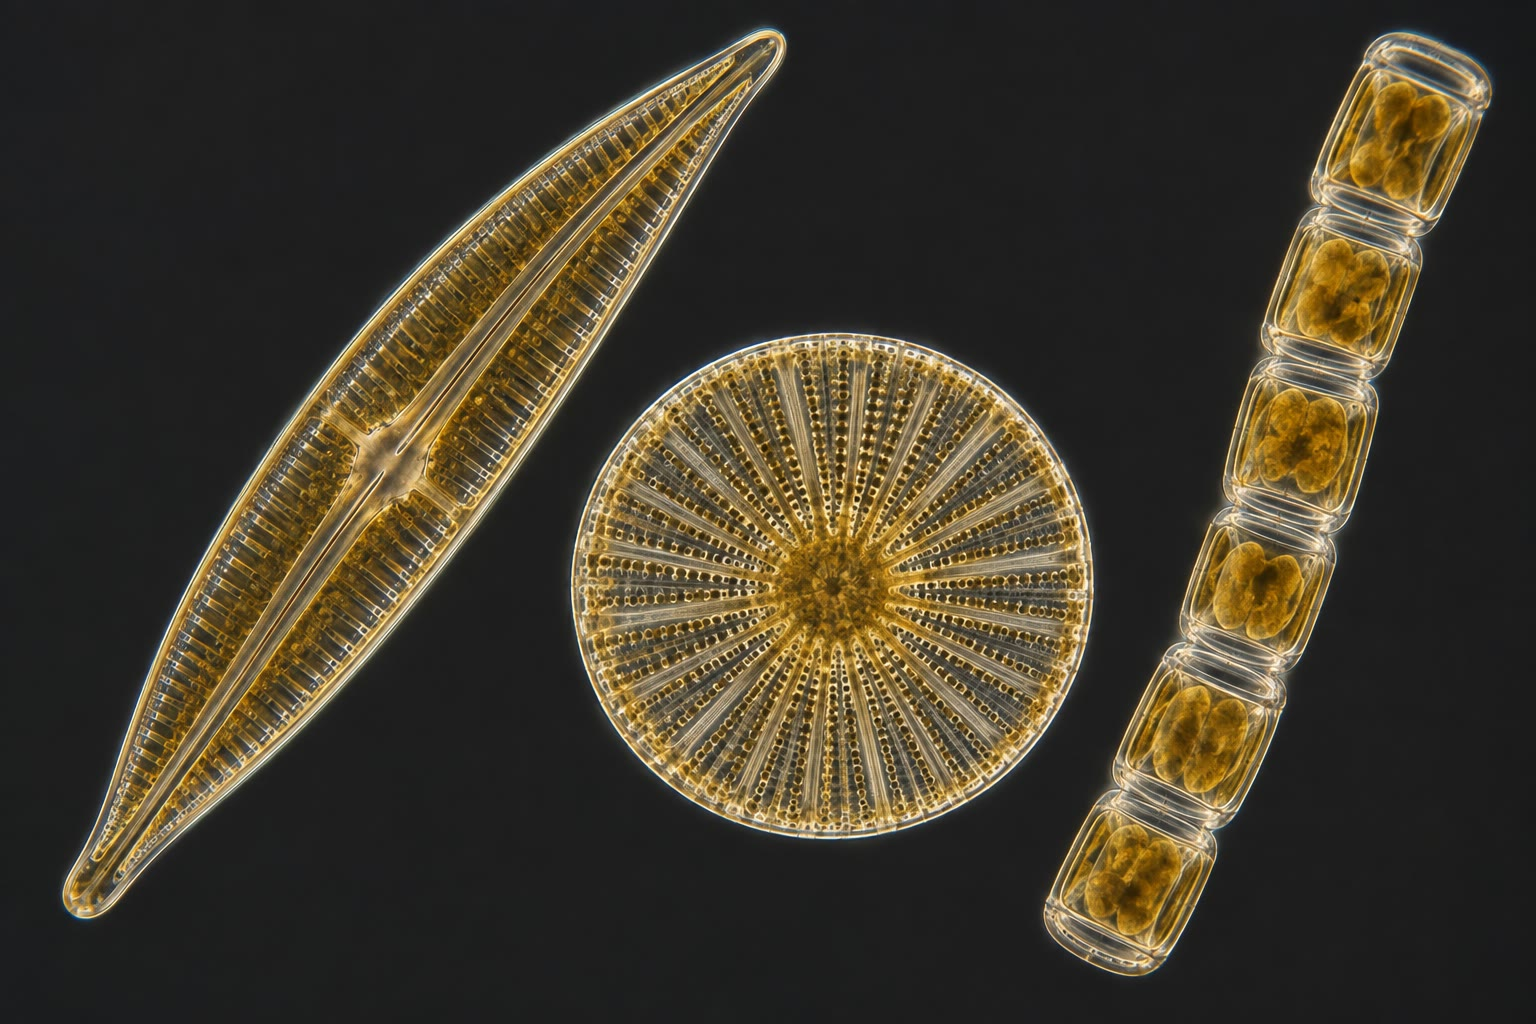
\includegraphics[width=0.6\linewidth]{images/book4/ai/b4-01-diatoms.jpg}

{\small 暗视野显微镜下的硅藻：每个细胞生活在
两片式的二氧化硅壳中，壳上布满小孔，细胞
借此与水交换物质。}
\end{omfigure}

\begin{definition}[营养方式]\label{def:b2:unicellular-diversity:nutrition}
\index{吞噬营养}\index{渗透营养}\index{混合营养生物}
单细胞真核生物以三种方式之一取食，或
同时采用其中两种。\emph{光能营养}：具有叶绿体，
以光和 $\mathrm{CO_2}$ 制造自身有机物（如绿藻、硅藻、
甲藻）。\emph{吞噬营养}：吞入颗粒物——
细菌、其他\omterm{def:b2:unicellular-diversity:protist}{原生生物}——吞入食物泡，其中
溶酶体酶将其消化（如变形虫、纤毛虫、领鞭毛虫）。
\emph{渗透营养}：经细胞膜吸收溶解的分子，
常先在体外分泌酶（如酵母及多种
寄生生物）。\emph{混合营养生物}，如 \emph{Euglena}，
在光照下进行光合作用，在黑暗中摄食。\omterm{def:b2:unicellular-diversity:prokaryote}{原核生物}不能吞噬：\omterm{def:b2:unicellular-diversity:prokaryote}{细胞壁}
禁止这样做，这正是\omterm{def:b2:unicellular-diversity:prokaryote}{原核生物}从未
靠吞入而成为捕食者的原因。
\end{definition}

\begin{proposition}[淡水中的渗透调节]\label{prop:b2:unicellular-diversity:osmoregulation}
\index{伸缩泡}
淡水\omterm{def:b2:unicellular-diversity:protist}{原生生物}体内比池水咸得多（溶质约 \qty{100}{mmol/L}，
池水约 \qty{1}{mmol/L}），且其细胞膜允许水通过。
因此水通过渗透作用持续进入细胞，
速率与表面积成正比，并与渗透压
差 $\Delta\Pi = RT\,\Delta c$ ——按上述数据
约为 \qty{2.4}{bar}。有\omterm{def:b2:unicellular-diversity:prokaryote}{细胞壁}的细胞靠
膨压抵抗；无壁细胞会在几分钟内膨胀破裂。
\emph{\omterm{prop:b2:unicellular-diversity:osmoregulation}{伸缩泡}}便是答案：一个由放射管供水的储库，
经质子驱动的转运蛋白泵入水分而充盈，
随后收缩，经一个小孔排出水分，每隔
几秒至几分钟一次。\emph{Paramecium} 每半小时
流经的水量相当于其自身体积；海洋近亲所处介质
与其自身一样咸，因而完全没有\omterm{prop:b2:unicellular-diversity:osmoregulation}{伸缩泡}。
\end{proposition}

\section{小型游动者的物理学}

\begin{proposition}[低雷诺数下的生命]\label{prop:b2:unicellular-diversity:reynolds}
\index{雷诺数}
\emph{\omterm{prop:b2:unicellular-diversity:reynolds}{雷诺数}} $Re = \rho v L/\eta$ 比较惯性力与黏性力，
用于尺寸为 $L$、以速度 $v$ 在密度为 $\rho$、黏度为 $\eta$ 的流体中运动的物体。
对人类游泳者，约为 $10^6$；
对 \emph{Paramecium}（\qty{200}{\micro m}，
\qty{1}{mm/s}）而言为 0.2，对细菌则为 $10^{-5}$。
低于 $Re \approx 1$ 时，惯性无关紧要：停止摆动的细胞
将在一纳米之内停止运动，水如同浓稠的糖浆，而
互易运动（同一动作向前和向后重复）不产生
净位移。因此，小型游动者采用非互易的动作：
细菌鞭毛的旋转螺旋、
纤毛不对称的摆动（僵硬的动力冲程与卷曲的恢复冲程），
以及 \emph{Chlamydomonas} 的蛙泳式划水。
\end{proposition}

\begin{theorem}[斯托克斯定律与沉降]\label{thm:b2:unicellular-diversity:stokes}
\index{斯托克斯定律}
半径为 $r$、密度为 $\rho_{\text{细胞}}$ 的球体在流体中缓慢运动时，
流体黏度为 $\eta$，它受到的阻力为 $F = 6\pi\eta r v$。
若任其自由地在密度为 $\rho$ 的水中，它将以终端
速度下沉：
\[
v_s = \frac{2\,r^2\,(\rho_{\text{细胞}} - \rho)\,g}{9\eta},
\]
沉降速度与半径的平方成正比：细胞大十倍，
下沉速度快一百倍。这就是浮游植物个体微小的原因，
也是硅藻带有刺和油滴的原因，同时解释了为何
\emph{Chlamydomonas} 停止游动后，会在
几天之内沉出光照层。
\end{theorem}
\begin{proof}
终端速度下，阻力与视重（重量
减去浮力）相平衡：$6\pi\eta r v_s = \tfrac{4}{3}\pi r^3
(\rho_{\text{细胞}} - \rho) g$。由此解出 $v_s$ 即得上式。
阻力定律本身在物理各册中推导，针对
$Re \ll 1$ 的情形；此处直接采用。
\end{proof}

\begin{example}[硅藻的下沉]\label{ex:b2:unicellular-diversity:fall}
半径为 \qty{10}{\micro m}、比海水密度大 \qty{100}{kg/m^3} 的中心硅藻
在海水（动力黏度 $\eta = \qty{1e-3}{Pa.s}$）中下沉，速度为
$v_s = 2\times 10^{-10}\times 100\times 9.81/(9\times 10^{-3}) =
\qty{2.2e-5}{m/s}$，约每天 \qty{2}{m}：它将在
不到一个月内离开 \qty{50}{m} 的光照层。其种群能够存续，
一是因为湍流搅动了水体，二是因为油滴与较低的密度
减小了 $\rho_{\text{细胞}} - \rho$，三是因为
下沉并在途中分裂的细胞所留下的后代
会被重新托起。
\end{example}

\begin{omfigure}
\begin{tikzpicture}
\begin{axis}[
  width=0.8\linewidth, height=6.0cm,
  axis x line=bottom, axis y line=left,
  xmode=log, ymode=log,
  xmin=0.5, xmax=200, ymin=1e-3, ymax=1e4,
  xlabel={半径（\unit{\micro m}）}, ylabel={下沉速度（\unit{\micro m/s}）},
  xlabel style={font=\small, at={(axis description cs:0.5,-0.1)}, anchor=north},
  ylabel style={font=\small},
  tick label style={font=\small},
  clip=false,
]
\addplot[very thick, omDef, domain=0.5:200, samples=40] {0.218*x^2};
\addplot[only marks, mark=*, mark size=1.8pt, omThm] coordinates {(1,0.218) (10,21.8) (100,2180)};
\node[font=\scriptsize, anchor=west] at (axis cs:1.15,0.218) {细菌};
\node[font=\scriptsize, anchor=west] at (axis cs:11.5,21.8) {硅藻};
\node[font=\scriptsize, anchor=east] at (axis cs:85,2180) {大型原生生物};
\end{axis}
\end{tikzpicture}

{\small 细胞的斯托克斯下沉速度随半径的变化，细胞密度比水大
\qty{100}{kg/m^3}。对数坐标下斜率为 2 即为
$r^2$ 律：细菌每天下沉约一厘米，大型
\omterm{def:b2:unicellular-diversity:protist}{原生生物}每小时下沉约两米。}
\end{omfigure}

\section{单细胞中的繁殖与性别}

\begin{definition}[分裂方式]\label{def:b2:unicellular-diversity:division}
\index{二分裂}\index{出芽}\index{复分裂}
\omterm{def:b2:unicellular-diversity:unicellular}{单细胞生物}通过分裂进行繁殖。\emph{二分裂}：细胞生长至
原来两倍大小，然后分裂为两个
等大的子细胞（见于细菌、\emph{Paramecium}、\emph{Amoeba}）。
\emph{出芽}：一个小的子细胞从母细胞长出并脱离
（酵母；母细胞保留一个痕迹，可出芽约二十次）。
\emph{复分裂}：细胞先长大，随后在母\omterm{def:b2:unicellular-diversity:prokaryote}{细胞壁}内
连续快速分裂数次，一次释放 4、8、
16 个或更多子细胞（见于 \emph{Chlamydomonas}，以及红细胞中的
疟原虫）。在恒定条件下，细胞数目
按指数规律增长，$N(t) = N_0\,2^{t/T}$，其中 $T$ 为
\emph{世代时间}\index{世代时间}：在丰富培养基中，
\emph{E.~coli} 约为二十分钟，许多藻类约为一天，某些纤毛虫约为一周。
（食物与生长的关系见
\cref{ch:b2:microbial-metabolism}。）
\end{definition}

\begin{proposition}[无繁殖的性：\emph{Paramecium} 中的接合]\label{prop:b2:unicellular-diversity:conjugation}
\index{接合!纤毛虫}
两个互补交配型的 \emph{Paramecium} 以口面相接。
在每个细胞中，二倍体小核进行减数分裂，形成
四个单倍体核，其中三个退化；存留的一个
进行有丝分裂，分为静止核和迁移核，两个
细胞通过连接处交换迁移核。每个细胞
随后将其静止核与接收到的迁移核融合，两个
伙伴分开，各自带有一个新的二倍体小核，其
基因型与伙伴相同。旧的大核解体，并
由新的小核重新形成一个大核。未产生新的细胞：
接合是基因混合——减数分裂与受精，见
\cref{ch:b2:meiosis-heredity}——与增殖脱钩。
细菌接合则不同，它将\omterm{def:b2:unicellular-diversity:prokaryote}{质粒}从供体
单向转移至受体，名称虽同，却是另一过程
（见\cref{ch:b2:genome-diversification}）。
\end{proposition}

\begin{omfigure}
\begin{tikzpicture}[every node/.style={font=\scriptsize}]
  \foreach \i/\x in {0/0,1/3.6,2/7.2,3/10.8} {
    \draw[thick, fill=omProp!8] (\x,0.55) ellipse (1.0 and 0.5);
    \draw[thick, fill=omProp!8] (\x,-0.55) ellipse (1.0 and 0.5);
  }
  % stage 0: two cells, diploid micronuclei 2n
  \fill[omDef!90!black] (0,0.55) circle (0.12); \node[right] at (0.15,0.55) {$2n$};
  \fill[omDef!90!black] (0,-0.55) circle (0.12); \node[right] at (0.15,-0.55) {$2n$};
  \node[below, align=center] at (0,-1.15) {两细胞相接};
  % stage 1: meiosis, 4 haploid, 3 degenerate
  \foreach \dy in {0.55,-0.55} {
    \fill[omDef!90!black] (3.6-0.3,\dy+0.15) circle (0.08);
    \fill[gray!60] (3.6+0.1,\dy+0.2) circle (0.06);
    \fill[gray!60] (3.6+0.3,\dy-0.05) circle (0.06);
    \fill[gray!60] (3.6-0.1,\dy-0.25) circle (0.06);
  }
  \node[below, align=center] at (3.6,-1.15) {减数分裂：\\4 个单倍体核，\\三个退化};
  % stage 2: mitosis, exchange
  \foreach \dy in {0.55,-0.55} {
    \fill[omDef!90!black] (7.2-0.35,\dy) circle (0.08);
    \fill[omThm] (7.2+0.35,\dy) circle (0.08);
  }
  \draw[->, thick, omThm] (7.55,0.45) -- (7.55,-0.45);
  \draw[->, thick, omThm] (6.85,-0.45) -- (6.85,0.45);
  \node[below, align=center] at (7.2,-1.15) {有丝分裂；迁移核（红色）\\相互交换};
  % stage 3: fusion 2n
  \fill[omDef!90!black] (10.8,0.55) circle (0.12); \node[right] at (10.95,0.55) {$2n$};
  \fill[omDef!90!black] (10.8,-0.55) circle (0.12); \node[right] at (10.95,-0.55) {$2n$};
  \node[below, align=center] at (10.8,-1.15) {受精：\\形成相同的二倍体核；\\细胞分开};
  \foreach \x in {1.3,4.9,8.5} \draw[->, thick, gray] (\x,0) -- (\x+1.0,0);
\end{tikzpicture}

{\small \emph{Paramecium} 的接合。两个细胞交换单倍体
核，然后分开，各自带有一个重组后的二倍体
小核；细胞数目没有改变。}
\end{omfigure}

\section{走向多细胞}

\begin{proposition}[团藻系列]\label{prop:b2:unicellular-diversity:volvox}
\index{Volvox@\emph{Volvox}}\index{多细胞性，起源}
在绿藻中，有一支谱系在现存物种中展示了
由单细胞到整体生物体的各个步骤。\emph{Chlamydomonas} 独居生活。
\emph{Gonium} 是一块扁平的板，由 4 至 16 个相同细胞组成，
它们一同游动。\emph{Pandorina} 和 \emph{Eudorina} 是中空的球，由 16
至 32 个细胞组成，细胞仍然完全相同，每个细胞都能建立一个新的群体。
\emph{Pleodorina} 有一些小细胞，它们只游动、从不
分裂。\omterm{prop:b2:unicellular-diversity:volvox}{\emph{Volvox}} 是一个球体，由 \num{500} 至 \num{50000} 个小的
体细胞，带有鞭毛，它们将随群体一同死亡，围绕着
少量大的生殖细胞，它们分裂形成子
球体，位于母球体之内。体细胞与生殖细胞就此出现：
这便是多细胞性的门槛，该谱系于
约 2 亿年前跨越了它，又独立地至少
在生命树的其他地方跨越了二十五次——包括动物、
植物、真菌、褐藻、红藻以及若干细菌类群。
\end{proposition}
\begin{proof}[证据]
由数十个基因构建的团藻类绿藻分子系统发生树表明，
\emph{Chlamydomonas} 位于基部，\omterm{prop:b2:unicellular-diversity:volvox}{\emph{Volvox}} 位于末端，
群体型类群介于两者之间，细胞数目
沿分支方向递增；\emph{Volvox carteri} 的基因组
（2010 年）与 \emph{Chlamydomonas} 的基因组相差几百个
基因，主要是维系细胞的细胞外基质的基因，
以及使体细胞停止分裂的调控基因。这一
转变所需的新遗传物质少得惊人。
\end{proof}

\begin{omfigure}
\begin{tikzpicture}[every node/.style={font=\scriptsize}]
  % Chlamydomonas
  \draw[thick, fill=omProp!25] (0,0) circle (0.22);
  \node[below=0.35cm, align=center] at (0,0) {\emph{Chlamydomonas}\\1 个细胞};
  % Gonium plate
  \begin{scope}[xshift=2.2cm]
    \foreach \x in {-0.3,0,0.3} \foreach \y in {-0.3,0,0.3} \draw[thick, fill=omProp!25] (\x,\y) circle (0.14);
    \draw[gray, dashed] (-0.55,-0.55) rectangle (0.55,0.55);
    \node[below=0.7cm, align=center] at (0,0) {\emph{Gonium}\\扁板，8--16 个细胞};
  \end{scope}
  % Eudorina ball
  \begin{scope}[xshift=4.5cm]
    \draw[gray, dashed] (0,0) circle (0.6);
    \foreach \a in {0,45,...,315} \draw[thick, fill=omProp!25] (\a:0.55) circle (0.13);
    \draw[thick, fill=omProp!25] (0,0.1) circle (0.13);
    \node[below=0.7cm, align=center] at (0,0) {\emph{Eudorina}\\32 个细胞的球，\\细胞完全相同};
  \end{scope}
  % Pleodorina
  \begin{scope}[xshift=7.4cm]
    \draw[gray, dashed] (0,0) circle (0.7);
    \foreach \a in {0,30,...,330} \draw[thick, fill=omProp!25] (\a:0.62) circle (0.09);
    \foreach \a in {60,180,300} \draw[thick, fill=omProp!60] (\a:0.62) circle (0.14);
    \node[below=0.8cm, align=center] at (0,0) {\emph{Pleodorina}\\部分细胞 \\只游动};
  \end{scope}
  % Volvox
  \begin{scope}[xshift=10.6cm]
    \draw[thick, fill=omProp!6] (0,0) circle (0.95);
    \foreach \a in {0,12,...,348} \fill[omProp!70] (\a:0.9) circle (0.035);
    \foreach \a in {0,12,...,348} \fill[omProp!50] (\a:0.72) circle (0.03);
    \foreach \p in {(0.25,0.2),(-0.3,-0.25),(0.1,-0.4),(-0.2,0.35)} \draw[thick, omThm, fill=omThm!40] \p circle (0.13);
    \node[below=1.05cm, align=center] at (0,0) {\emph{Volvox}\\数千个体细胞 \\和少量生殖细胞（红色）};
  \end{scope}
  \foreach \x in {0.5,3.0,5.3,8.3} \draw[->, gray] (\x,0) -- (\x+0.6,0);
\end{tikzpicture}

{\small 团藻系列：单细胞、扁平板、由相同细胞组成的空心球，
其中部分细胞已放弃
分裂的球，以及 \omterm{prop:b2:unicellular-diversity:volvox}{\emph{Volvox}}，其中数千个会死亡的体细胞
包围着少量生殖细胞。}
\end{omfigure}

\begin{omfigure}
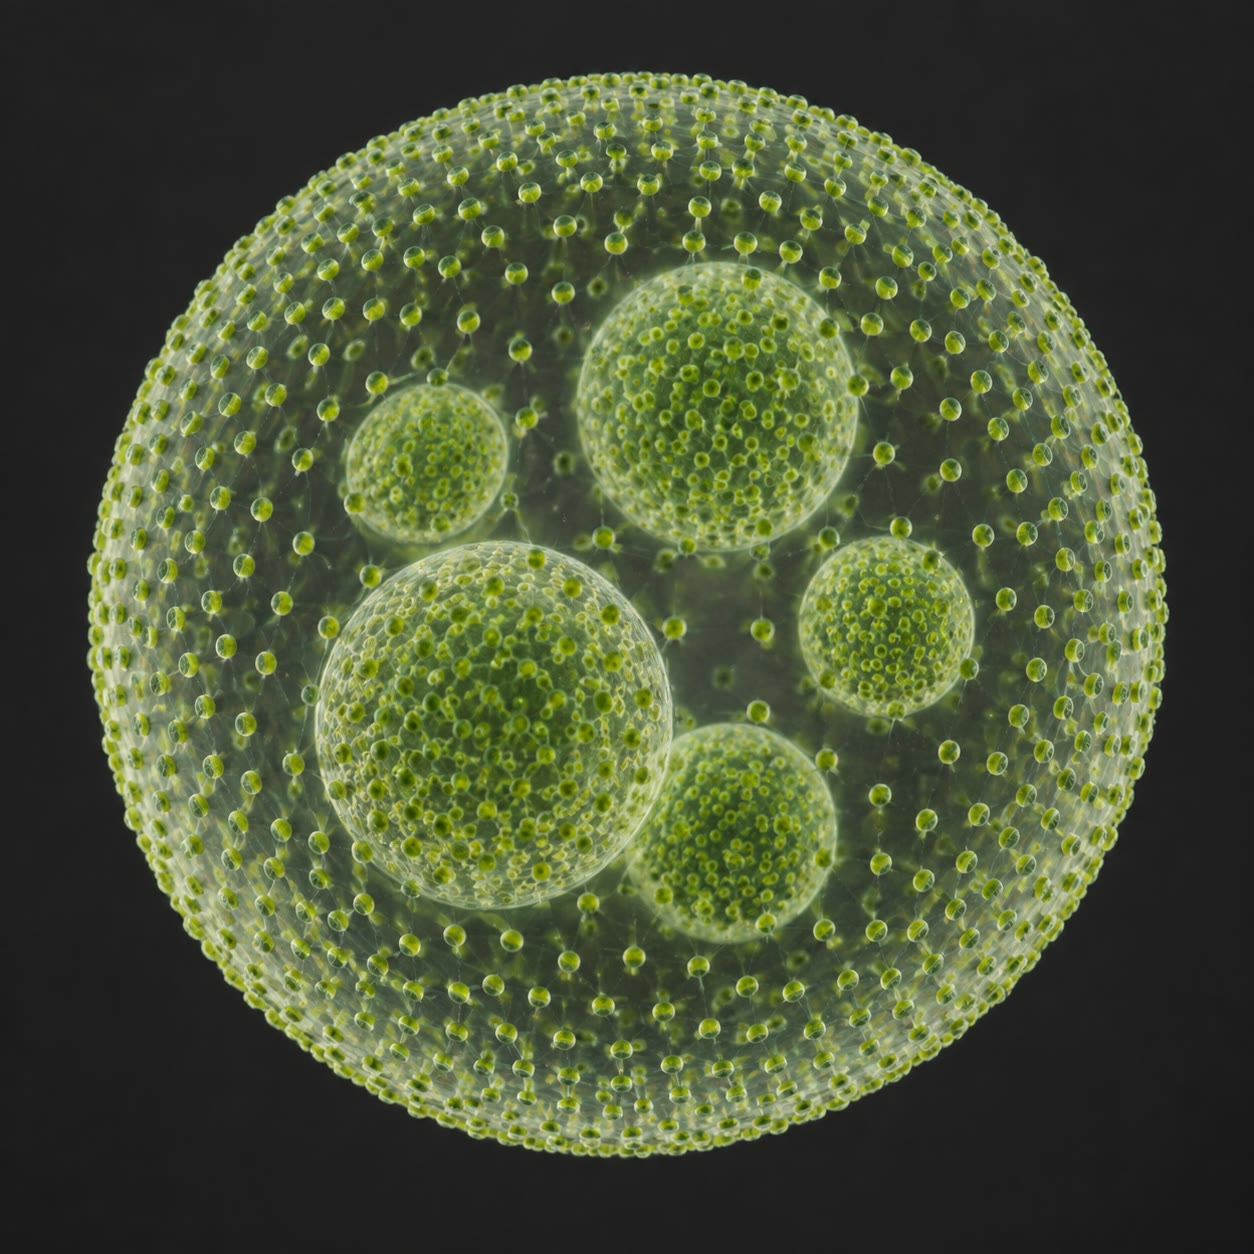
\includegraphics[width=0.55\linewidth]{images/book4/ai/b4-01-volvox.jpg}

{\small 一个 \omterm{prop:b2:unicellular-diversity:volvox}{\emph{Volvox}} 群体：中空的绿色球体，由带鞭毛的
细胞构成，内部生长着子群体。}
\end{omfigure}

\begin{remark}[为何要分工？]\label{rem:b2:unicellular-diversity:whydivide}
在这些藻类中，一个细胞不能同时游动与分裂：
锚定鞭毛的基体，是组织
纺锤体所必需的。单细胞轮流进行两者；小群体可以
停止游动，让所有细胞同时分裂；大群体则会下沉
出光照范围（斯托克斯定律，见\cref{thm:b2:unicellular-diversity:stokes}）
在其分裂所需的数小时之内。超过一定大小后，
让部分细胞继续游动、其余细胞分裂，便值得牺牲它们的
后代——体细胞由此诞生。襟鞭毛虫是一类具领的
鞭毛虫，其细胞与海绵的摄食细胞相同，
在通向动物的那一支上展示了同样的最初几步。
\end{remark}

\section{练习}

\begin{exercise}[$\star$]\label{exo:b2:unicellular-diversity:1}
给出单细胞、群体的与多细胞的定义，并将
\emph{E.~coli}、\emph{Gonium}、\omterm{prop:b2:unicellular-diversity:volvox}{\emph{Volvox}} 和一个酵母细胞分别
归入正确的类别，并说明理由。
\end{exercise}

\begin{exercise}[$\star$]\label{exo:b2:unicellular-diversity:2}
计算半径为
\qty{0.5}{\micro m} 的球菌，以及半径为
\qty{50}{\micro m} 的球形\omterm{def:b2:unicellular-diversity:protist}{原生生物}的\omterm{prop:b2:unicellular-diversity:surface}{表面积与体积之比}。哪一个每单位
细胞质的呼吸更快，为什么？
\end{exercise}

\begin{exercise}[$\star$]\label{exo:b2:unicellular-diversity:3}
给出细菌与单细胞真核生物之间的
三个结构差异，以及细菌不能做、
而变形虫能做的一件事。
\end{exercise}

\begin{exercise}[$\star$]\label{exo:b2:unicellular-diversity:4}
说出下列
\emph{Paramecium} 各结构的功能：纤毛、口沟、食物泡、\omterm{prop:b2:unicellular-diversity:osmoregulation}{伸缩泡}、
大核、小核。
\end{exercise}

\begin{exercise}[$\star\star$]\label{exo:b2:unicellular-diversity:5}
已知细胞质中某代谢物的 $D = \qty{5e-10}{m^2/s}$，求扩散穿过
\qty{1}{\micro m} 的细菌与 \qty{500}{\micro m} 的变形虫各需多长时间？
请评论变形虫必须做到、而细菌无需做到的
事情。
\end{exercise}

\begin{exercise}[$\star\star$]\label{exo:b2:unicellular-diversity:6}
计算 \emph{Paramecium}（\qty{200}{\micro
m}, \qty{1}{mm/s}）、细菌（\qty{2}{\micro m}, \qty{20}{\micro
m/s}）与人类游泳者（\qty{2}{m}, \qty{1}{m/s}）的\omterm{prop:b2:unicellular-diversity:reynolds}{雷诺数}，
取 $\rho = \qty{1000}{kg/m^3}$ 与 $\eta = \qty{1e-3}{Pa.s}$。
为何游泳者一次划水之后还能滑行，而细菌不能？
\end{exercise}

\begin{exercise}[$\star\star$]\label{exo:b2:unicellular-diversity:7}
一个半径为 \qty{10}{\micro m} 的硅藻，
比水的密度大 \qty{100}{kg/m^3}。求其下沉速度，以及下落
\qty{50}{m} 所需的时间。若细胞半径减半，时间将变为原来的多少倍？
若它将超出水的那部分密度削减至 \qty{20}{kg/m^3}，又如何？
\end{exercise}

\begin{exercise}[$\star\star$]\label{exo:b2:unicellular-diversity:8}
将 \emph{Paramecium} 近似为半轴分别为 \num{100}、
\num{25} 与 \qty{25}{\micro m} 的椭球体（$V = \tfrac{4}{3}\pi abc$）。它
每 \qty{30}{min} 排出一个与自身体积相等的水量。求
水的内流量，分别以 \unit{\micro m^3/s} 和升每秒表示。
\end{exercise}

\begin{exercise}[$\star\star$]\label{exo:b2:unicellular-diversity:9}
某引诱剂在 \qty{1}{mm} 内浓度加倍。求
\qty{1}{\micro m} 的细菌两端之间的相对差异；
以 \qty{20}{\micro m/s} 的速度游动 \qty{1}{s} 时，起点与终点之间的相对差异又是多少？
对 $N$ 个分子计数的相对误差约为 $1/\sqrt{N}$：
试说明细菌为何比较时间，而非比较
两侧的浓度。
\end{exercise}

\begin{exercise}[$\star\star\star$]\label{exo:b2:unicellular-diversity:10}
\emph{Thiomargarita namibiensis} 是一种球形硫细菌，
直径为 \qty{500}{\micro m}，细胞质呈
厚 \qty{2}{\micro m} 的壳层，环绕一个硝酸盐液泡。求其
表面积与\emph{细胞质}体积之比，并与
\emph{E.~coli}（半径为 \qty{0.5}{\micro m} 的圆柱，忽略两端）相比。说明
液泡如何使其能长得如此之大，
以及硝酸盐的作用是什么。
\end{exercise}

\begin{exercise}[$\star\star\star$]\label{exo:b2:unicellular-diversity:11}
在 \omterm{prop:b2:unicellular-diversity:volvox}{\emph{Volvox}} 中，体细胞从不分裂，并随群体
一同死亡。利用鞭毛约束与斯托克斯定律，
说明为何此类细胞在含 \num{10000} 个细胞的群体中值得拥有，
而在仅 16 个细胞的群体中则不然，并说明为何生殖细胞
是球体中最大的细胞。
\end{exercise}

\begin{exercise}[$\star\star\star$]\label{exo:b2:unicellular-diversity:12}
“\omterm{def:b2:unicellular-diversity:protist}{原生生物}是一个演化级，而不是演化支。”结合本章提到的
谱系说明二者的区别，并说明为何同样的说法对“\omterm{def:b2:unicellular-diversity:prokaryote}{原核生物}”成立，
而对“蓝细菌”不成立。
\end{exercise}

\section{问题：一滴池塘水}

\begin{problem}[{周末问题——对一份池塘水样进行计数、培养，
并分析支配其细胞的物理规律，最后落到
一种绿藻的水与能量收支}]
\label{pb:b2:unicellular-diversity:1}
于春季对一个体积为 \qty{1000}{m^3} 的池塘取样。在显微镜下，
一个计数室，其网格面积为 \qty{1}{mm}$\times$\qty{1}{mm}，
盖玻片位于其上方 \qty{0.1}{mm}，视野中可见 24 个
\emph{Chlamydomonas}（半径为 \qty{5}{\micro m} 的球体，
密度为 \qty{1050}{kg/m^3}）。取 $\rho = \qty{1000}{kg/m^3}$，
$\eta = \qty{1e-3}{Pa.s}$，$g = \qty{9.81}{m/s^2}$，$R =
\qty{8.314}{J/mol/K}$，$T = \qty{293}{K}$，$D = \qty{1.9e-9}{m^2/s}$
为 $\mathrm{CO_2}$ 在水中的扩散系数。

\medskip
\noindent\textbf{第一部分——计数。}
\begin{enumerate}
  \item 计算网格下方水的体积，以微升计。
  \item 推算池塘中 \emph{Chlamydomonas} 的密度，
        以每毫升的细胞数表示。
  \item 计算单个细胞的体积，以及\omterm{prop:b2:unicellular-diversity:surface}{表面积与
        体积之比}。
  \item 池塘水体积中被这些细胞占据的
        比例是多少？
  \item 池塘中共有 \emph{Chlamydomonas} 多少个？
  \item 池塘中还有一种丝状蓝细菌。给出两个
        在显微镜下可见的、能够将其
        与该藻类区分开的特征。
\end{enumerate}

\medskip
\noindent\textbf{第二部分——生长。}
样品置于光照下，\qty{48}{h} 后再次计数：
在网格下计得 \num{384} 个细胞。
\begin{enumerate}[resume]
  \item 计算\omterm{def:b2:unicellular-diversity:division}{世代时间} $T$。
  \item 计算增长速率常数 $k$（在 $N = N_0 e^{kt}$ 中），
        单位为 \unit{h^{-1}}。
  \item 若按此速率，池塘种群需多长时间才能达到
        每毫升 \qty{1e8}{} 个细胞？
  \item 给出它不会如此增长的三个理由。
  \item 若细胞仅在白天的 \qty{12}{h} 内生长，
        夜间完全不生长，同样的增长需多长时间？
  \item \emph{Chlamydomonas} 通过\omterm{def:b2:unicellular-diversity:division}{复分裂}繁殖，一次释放
        4、8 或 16 个子细胞。试说明为何\omterm{def:b2:unicellular-diversity:division}{世代时间}
        仍可由计数明确界定。
\end{enumerate}

\medskip
\noindent\textbf{第三部分——细胞的物理学。}
\begin{enumerate}[resume]
  \item 计算一个以
        \qty{100}{\micro m/s} 的速度游动的细胞的\omterm{prop:b2:unicellular-diversity:reynolds}{雷诺数}。
  \item 质量为 $m$ 的细胞停止摆动鞭毛后，
        依惯性滑行的距离为 $mv/(6\pi\eta r)$。计算该距离。
  \item 计算已停止
        游动的细胞的下沉速度。
  \item 比较下沉 \qty{1}{m} 所需的时间，
        与向上游动 \qty{1}{m} 所需的时间。
  \item 池塘中溶解有 \qty{10}{\micro mol/L}
        的 $\mathrm{CO_2}$，计算细胞能获得的最大扩散供应，
        以每秒的 $\mathrm{CO_2}$ 分子数计。
  \item 一个细胞含有 \qty{100}{pg} 的碳，一个世代内
        碳量加倍。计算其平均碳需求（以分子每秒计），
        并求供应与需求之比。
  \item 对一假想细胞（半径为
        \qty{50}{\micro m}，碳密度相同）重做比较，并作出结论。
\end{enumerate}

\medskip
\noindent\textbf{第四部分——水与能量。}
细胞质中含有 \qty{100}{mmol/L} 溶质，池塘中含
\qty{1}{mmol/L}。膜的水力传导率为 $L_p =
\qty{1e-14}{m.s^{-1}.Pa^{-1}}$（单位面积上、单位压差下的水体积通量）。
水解一个 ATP 可释放的能量为
\qty{50}{kJ/mol}；固定一个碳原子需消耗三个 ATP。
\begin{enumerate}[resume]
  \item 计算膜两侧的渗透压差。
  \item 计算每秒进入细胞的水的体积，
        单位为 \unit{\micro m^3/s}。
  \item 若无\omterm{prop:b2:unicellular-diversity:osmoregulation}{伸缩泡}，该细胞需多长时间
        才能使其体积加倍？
  \item 计算逆着渗透压排出这些水所需的
        最小功率。
  \item 将其换算为每秒 ATP 分子数，并与
        细胞用于碳固定的 ATP 量（见问题 18）比较。
  \item 给出结论：细胞的水内流量、
        胀破所需时间，以及维持细胞“干燥”
        所耗能量占其总能量的比例。
\end{enumerate}
\end{problem}
